\section{Introduction}
The goal of the assignment is to implement an interactive application in D3 to visualize the data we got for this assignment. We received a dataset with data from all municipalities in the Netherlands.  We were asked to look carefully at this data and derive which aspects of the data could be of interest for the analyst. We will describe the interesting parts of the data in section~\ref{Sec:Dat}. Of course the interesting aspects of the data are hard to analyze from the raw data, so we were asked to think of multiple ways in how to visualize these aspects of the data. In section~\ref{Sec:Des} we will describe the visualization techniques and the pros of cons of these visualization techniques and how these techniques work combined. For readers that are interested in making a D3 implementation themselves, we will describe how we implemented all parts of the application in section~\ref{Sec:Imp}. At last we will evaluate how well the application works for the tasks we thought that were interesting. This will be described in section~\ref{Sec:Dis}.
\begin{figure}[H]
					\centering
						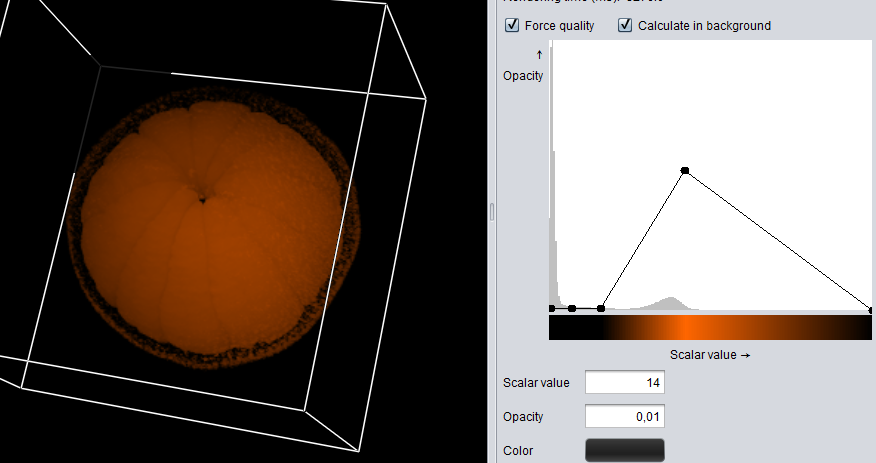
\includegraphics[width=\textwidth]{{img/intro_app}}
						\caption{Overview of our application, showing some provinces expanded and some not. There has also been zoomed in to show more details on Renkum}
						\label{fig:intro}
	\end{figure}
